\section{Ejercicio 8 - Definir indicadores clave de rendimiento (KPI)}  

1.Cambiarse a la pestaña KPI La pestaña KPI incluye varios paneles. En la parte izquierda de la pestaña están el panel Organizador de KPI y el panel Herramientas de cálculo. El panel de muestra del centro de la pestaña contiene los detalles del KPI seleccionado en el panel Organizador de KPI. La siguiente imagen muestra la pestaña KPI del Diseñador de cubos

	\begin{center}
	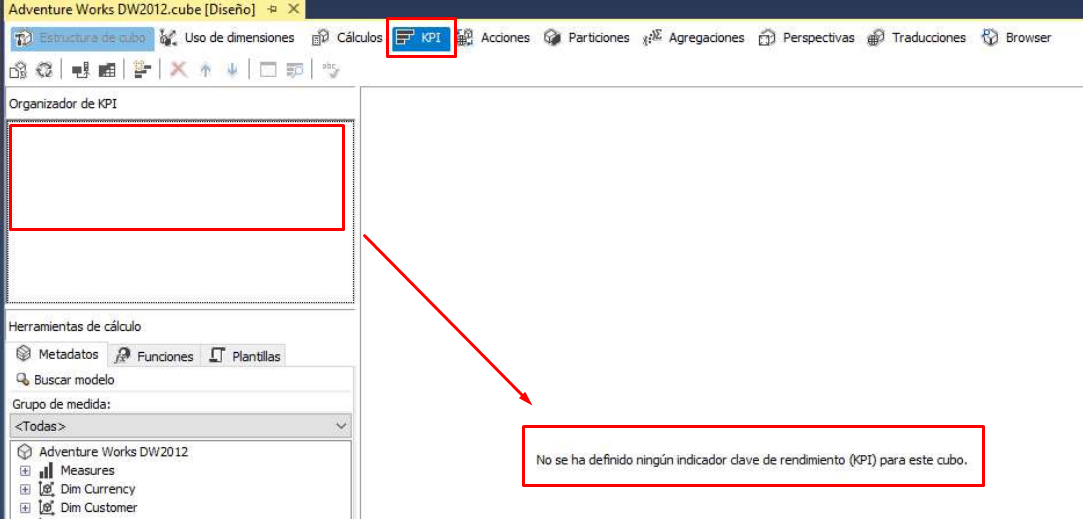
\includegraphics[width=\columnwidth]{images/task8/img1}
	\end{center}	

2. En la barra de herramientas de la pestaña KPI, haga clic en el botón Nuevo KPI en el panel de muestra aparecerá una plantilla de KPI en blanco, como en la siguiente imagen.

	\begin{center}
	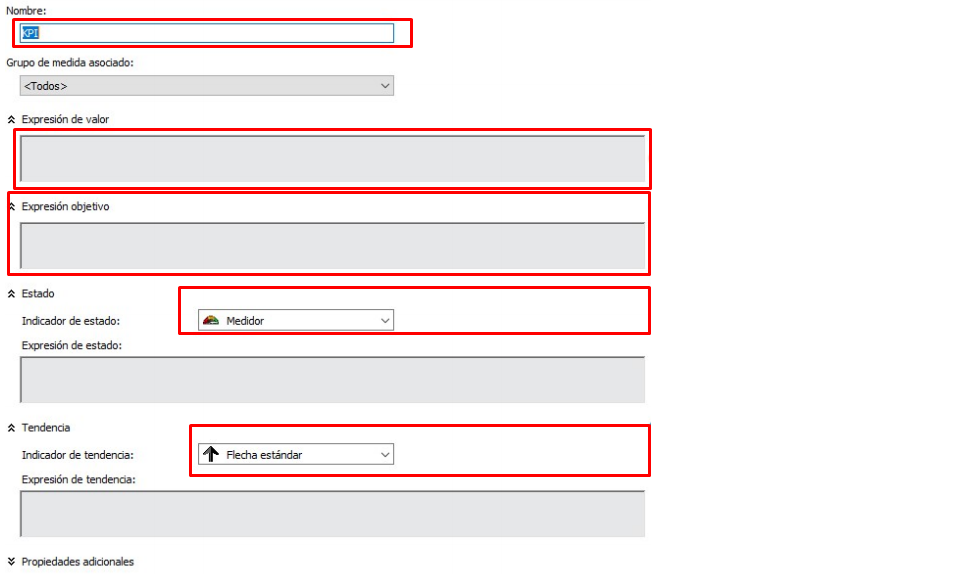
\includegraphics[width=\columnwidth]{images/task8/img2}
	\end{center}	

3. En el cuadro Nombre, escriba Venta y, a continuación, seleccione Fact Internet Sales en la lista Grupo de medida
asociado

4. En la pestaña Metadatos del panel Herramientas de cálculo, expanda Medidas

	\begin{center}
	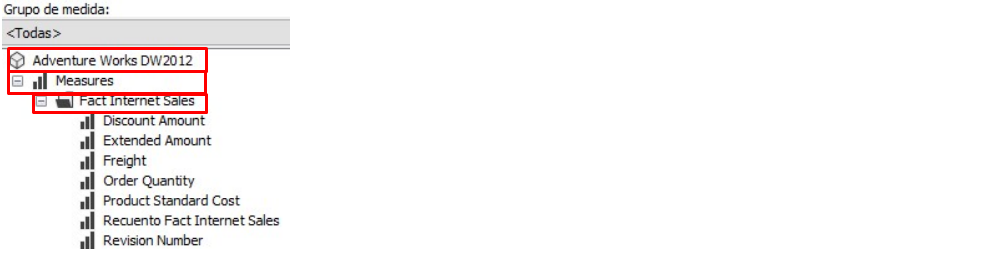
\includegraphics[width=\columnwidth]{images/task8/img3}
	\end{center}	


5. Expanda la tabla Fact Internet Sales y, a continuación, arrastre la medida Sales Amount al cuadro Expresión de
valor.

	\begin{center}
	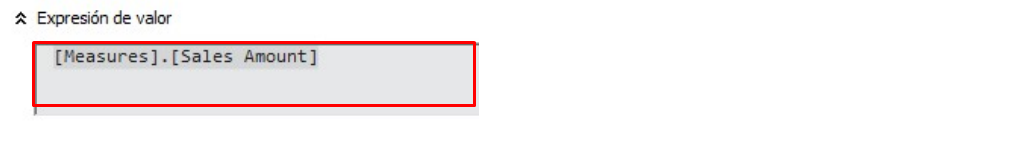
\includegraphics[width=\columnwidth]{images/task8/img4}
	\end{center}	


6. En el cuadro Expresión objetivo digite:

	\begin{center}
	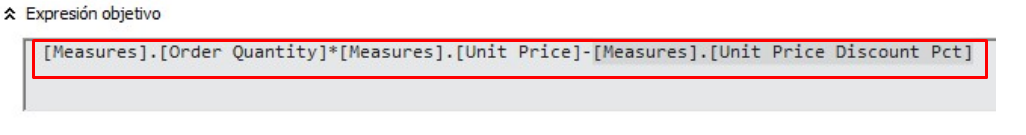
\includegraphics[width=\columnwidth]{images/task8/img5}
	\end{center}	

7. Compruebe que está seleccionado Indicador en la lista Indicador de estado, seleccione uno tal como se muestra
en la figura:

	\begin{center}
	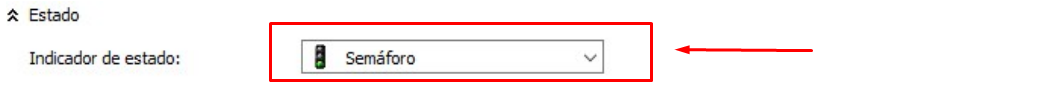
\includegraphics[width=\columnwidth]{images/task8/img6}
	\end{center}	

y, a continuación, escriba la siguiente expresión MDX en el cuadro Expresión de estado:

	\begin{center}
	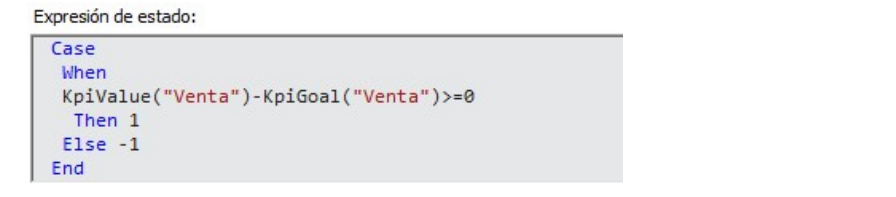
\includegraphics[width=\columnwidth]{images/task8/img7}
	\end{center}	


8. Compruebe que está seleccionado Flecha estándar en la lista Indicador de tendencia

	\begin{center}
	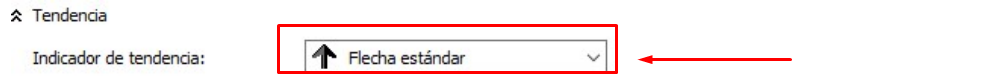
\includegraphics[width=\columnwidth]{images/task8/img8}
	\end{center}	

9. Y a continuación, escriba la siguiente expresión en el cuadro Expresión de tendencia:

	\begin{center}
	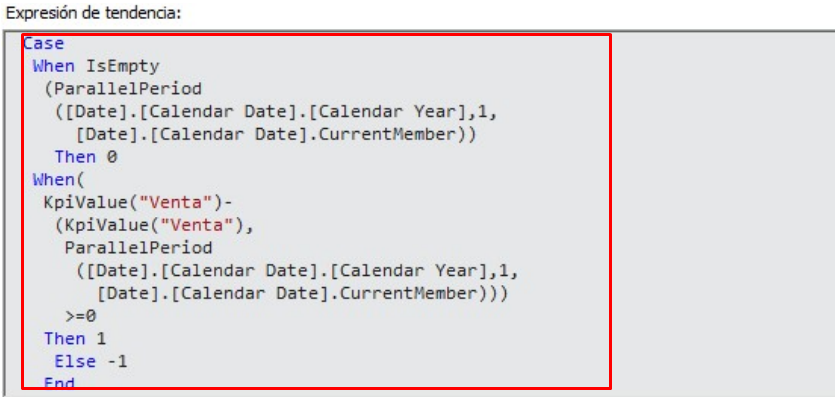
\includegraphics[width=\columnwidth]{images/task8/img9}
	\end{center}	


10. Guardar los cambios

11. Cerrar el diseñador del cubo

12. Procesar el cubo

\subsection{Examinar el cubo mediante el KPI}

1. Abrir el diseñador del cubo

2. Hacer clic en la pestaña KPI

	\begin{center}
	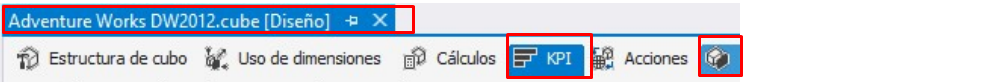
\includegraphics[width=\columnwidth]{images/task8/img10}
	\end{center}	

3. Luego haga clic en la opción Vista examinador.

4. En el panel Filtro, seleccione Order Date en la lista Dimensión

5. Seleccione Calendar Date en la lista Jerarquía, seleccione Igual en la lista Operador

	\begin{center}
	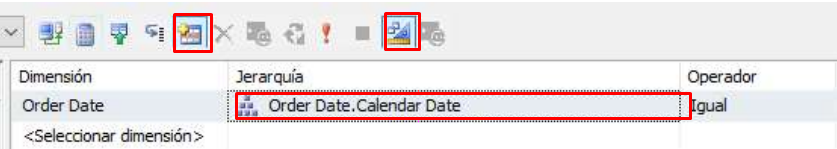
\includegraphics[width=\columnwidth]{images/task8/img11}
	\end{center}	

6. En la lista Expresión de filtro seleccione tal como se muestra a continuación:

	\begin{center}
	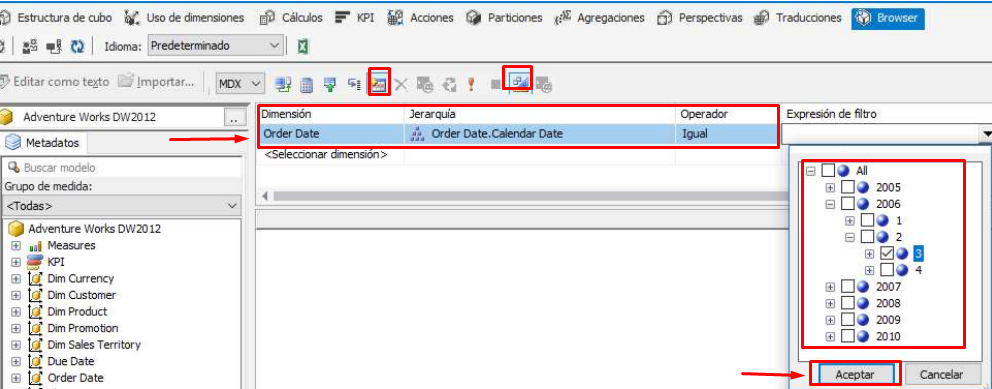
\includegraphics[width=\columnwidth]{images/task8/img12}
	\end{center}	

7. Y a continuación, haga clic en Aceptar

8. Arrastre el KPI al panel Examinador de KPI

	\begin{center}
	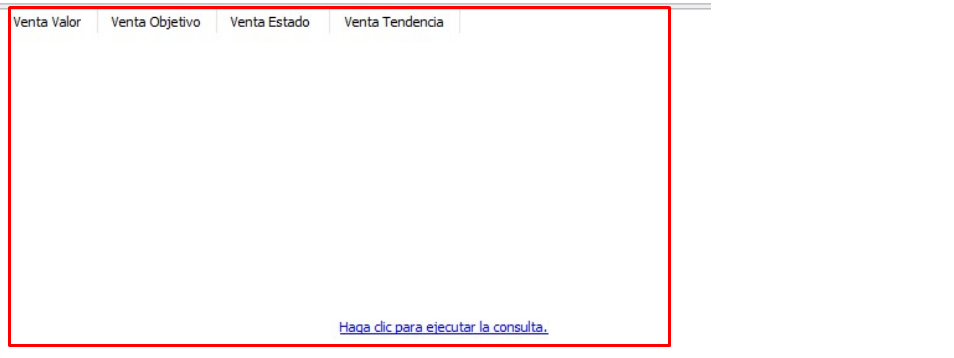
\includegraphics[width=\columnwidth]{images/task8/img13}
	\end{center}	

9. Para actualizar los valores para el KPI Venta, haga clic en el enlace “Haga clic para ejecutar la consulta”


	\begin{center}
	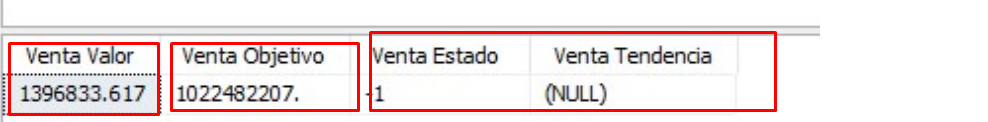
\includegraphics[width=\columnwidth]{images/task8/img14}
	\end{center}	